

\chapter{Ορισμός του Προβλήματος και Στρατηγικές Επίλυσης} \label{ch:strategies_solution}
Στο κεφάλαιο αυτό, θα παρουσιαστεί το μοντέλο κάτω από το οποίο γίνονται οι υπολογισμοί και αφού οριστεί το πρόβλημα με μαθηματικούς ορισμούς, θα αποδειχθεί οτι το
πρόβλημα ανήκει στην κλάση NP-πλήρης (NP-Complete) των προβλημάτων, δηλαδή δεν υπάρχει πολυωνιμικός αλγόριθμος που να το λύνει. Θα αποδειχθεί ένα άνω φράγμα του
προβλήματος βασισμένο στον γραμμικό προγραμματισμό (linear programming) ενώ θα παρουσιαστούν παρόμοιες εργασίες οι οποίες όμως μέχρι τώρα διαφέρουν ως προς την
προσέγγιση του προβλήματος σε σχέση με την παρούσα εργασία. Τέλος θα προταθούν ευρετικές στρατηγικές που αυξάνουν την απόδοση του φορτιστή αλλά και ευρετικοί
αλγόριθμοι τοπικής και καθολικής γνώσης οι οποίοι θα συγκριθούν με έναν προσαρμοστικός αλγόριθμο ο οποίος ρυθμίζει την διαδρομή του φορτιστή ανάλογα με την κατάσταση
του δικτύου.


\section{Γενικευμένος Ορισμός, Μοντέλο Επίλυσης και Ιδιότητες}
Στην ενότητα αυτή παρουσιάζεται ο γενικευμένος ορισμός του προβλήματος ο οποίος δεν αφορά μόνο την τεχνολογία ασύρματης μετάδοσης ενέργειας. Αντίθετα το πρόβλημα
ορίζεται κάτω από την γενικότερη έννοια της επαναφόρτισης των κόμβων, είτε αυτή είναι ασύρματη, είτε είναι ενσύρματη. Επίσης, ορίζεται αυστηρά το μοντέλο κάτω από το
οποίο θα παρουσιαστούν οι λύσεις του προβλήματος. Είναι σημαντικό το μοντέλο να είναι απλό ώστε να είναι εύκολα δυνατό να γίνουν αναλύσεις και να εξαχθούν λύσεις
αλλά θα πρέπει ταυτόχρονα το μοντέλο να αντικατοπτρίζει την πραγματικότητα, δηλαδή να έχει άμεση σχέση με το φυσικό περιβάλλον. Στην συνέχεια αποδεικνύεται οτι το
πρόβλημα αυτό ανήκει στην κλάση των προβλημάτων που είναι NP-πλήρη (NP-complete), δηλαδή είναι υπολογιστικά δύσκολο να βρεθεί γρήγορα μια λύση.

\subsection{Γενικευμένος Ορισμός}
Οι καινούργιες τεχνολογίες που αναλύθηκαν στην ενότητα $\ref{sc:recharg_tecnhiques}$ οδηγούν σε νέες ερευνητικές προκλήσεις των ασύρματων δικτύων αισθητήρων. Ο πλέον
μεγάλος περιορισμός των υπάρχοντων τεχνολογιών είναι εκείνος της περιορισμένης ενέργειας. Όμως, με τις πρόσφατες εξελίξεις στην τεχνολογία της ασύρματης μετάδοσης
ενέργειας, ο διαχειρισμός της ενέργειας σε τέτοιου είδους δίκτυα είναι σημαντικός. Μια αποδοτική διαχείρηση ενέργειας μπορεί να οδηγήσει σε καλύτερα αποτελέσματα ως
προς όλες τις μετρικές των ΑΔΑ (ενότητα $\ref{sc:wsn_design}$). Επίσης αυτή η διαχείρηση ενέργειας στα ΑΕΔΑ θα πρέπει γίνεται παθητικά ως προς τους στατικούς κόμβους,
δηλαδή δεν χρειάζεται καινούργιο πολύπλοκο πρωτόκολο γι'αυτή την διαχείρηση που να καταναλώνει επιπλέον ενέργεια στους στατικούς κόμβους, ενώ ταυτόχρονα ιδανικά θα
πρέπει να είναι και ανεξαρτήτου του πρωτοκόλου δρομολόγησης που χρησιμοποιείται. Ο γενικευμένος ορισμός του προβλήματος παρουσιάζεται στην συνέχεια:

\textbf{Το Πρόβλημα:} \textit{Έστω ένα ασύρματα επαναφορτιζόμενο δίκτυο αισθητήρων το οποίο αποτελείται από ένα σύνολο στατικών κόμβων και έναν ειδικό κινητό κόμβο,
τον κινητό φορτιστή. Οι στατικοί κόμβοι τοποθετούνται ομοιόμορφα κατανεμημένα στην περιοχή του δικτύου και διαδίδουν τα δεδομένα τους, σύμφωνα με ένα πρωτόκολλο
δρομολόγησης, προς την Πηγή, η οποία βρίσκεται στο κέντρο του δικτύου. Ο κινητός φορτιστής έχει πεπερασμένους πόρους ενέργειας οι οποίοι όμως είναι σημαντικά
μεγαλύτεροι από τους πεπερασμένους πόρους ενέργειας των στατικών κόμβων ενώ ταυτόχρονα είναι ικανός να φορτίζει τους φορτίζει. Το πρόβλημα που μελετάται είναι ο
προσδιορισμός της βέλτιστης δυνατής διαμόρφωσης όλων των παραμέτρων του δικτύου έτσι ώστε να βελτιωθεί η απόδοτικότητα και να αυξηθεί ο χρόνος ζωής του δικτύου.}

\textit{Οι παράμετροι που θα μελετηθούν είναι η πολιτική φόρτισης του κάθε στατικού κόμβου (δηλαδή αν ο κινητός φορτιστής τον φορτίζει ολικώς ή μερικώς), η αναλογία
της ενέργειας που είναι αρχικά διαθέσιμη στον κινητό φορτιστή και στους στατικούς κόμβους, καθώς και οι βέλτιστες διαδρομές που θα ακολουθεί ο κινητός φορτιστής ως
προς την απόδοση και την αύξηση του χρόνου ζωής του δικτύου.}



\subsection{Μοντέλο Ανάπτυξης, Ενέργειας και Φόρτισης Κόμβων}
Το μοντέλο του προβλήματος, από τον ορισμό του, περιέχει 3 τύπους συσκευών. Υπάρχουν $N$ στατικοί κόμβοι (αισθητήρες) ομοιόμορφα κατανεμημένοι στο δίκτυο οι
οποίοι επιβλέπουν το περιβάλλον και ανιχνεύουν διάφορα γεγονότα που γίνονται σε αυτό. Οι στατικοί κόμβοι έχουν αρκετή υπολογιστική ισχύ για να εκτελέσουν βασικές
εφαρμογές των ασύρματων δικτύων αισθητήρων αλλά ταυτόχρονα έχουν περιορισμένους πόρους όσον αφορά την αποθήκευση της ενέργειας. Στην συνέχεια υπάρχει ένας κινητός
κόμβος, ο κινητός φορτιστής $MC$, ο οποίος θεωρούμε οτι έχει και αυτός πεπερασμένη διαθέσιμη ενέργεια αλλά πολύ μεγαλύτερη από αυτή που έχουν οι στατικοί κόμβοι.
Τέλος υπάρχει η Πηγή $S$, η οποία βρίσκεται στο κέντρο του δικτύου και είναι ο κόμβος στον οποίο καταλήγουν όλα τα πακέτα των στατικών κόμβων. Θεωρούμε οτι η Πηγή
έχει άπειρα υπολογιστική ισχύ και άπειρη ενέργεια. Επίσης θεωρείται οτι το δίκτυο είναι ένας κυκλικός δίσκος ακτίνας $R$. Η ακτίνα επικοινωνίας των κόμβων, έστω $r$
ποικίλει ανάλογα με το πρωτόκολλο δρομολόγησης που χρησιμοποιείται. Η πυκνότητα του δικτύου είναι:
\begin{align*}
\rho = \frac{N}{\pi\cdot R^{2}}
\end{align*}

Στο μοντέλο ο κινητός φορτιστής $MC$ δεν συλλέγει δεδομένα από τους κόμβους αλλά μόνο τους φορτίζει. Επίσης χάρην απλότητας θεωρείται οτι όλοι οι
κόμβοι έχουν την ίδια συχνότητα παραγωγής μηνυμάτων, έστω $\lambda$ πακέτα ανά μονάδα χρόνου. Επιπλέον Θεωρείται οτι $E_{total}$ είναι η συνολική διαθέσιμη ενέργεια
που μπορούμε να βάλουμε στο δίκτυο, είτε δοθεί όλη στους στατικούς κόμβους είτε την μοιράστεί ανάμεσα στους στατικούς κόμβους και τον κινητό φορτιστή. Δηλαδή
αρχικά είναι:
\begin{align}
\label{total}
E_{total} = E_{sensors} + E_{MC}^{init}
\end{align}
όπου $E_{sensors}$ είναι η αρχική ενέργεια που δίνεται στους στατικούς κόμβους και $E_{MC}^{init}$ η αρχική ενέργεια που δίνεται στον κινητό φορτιστή. Η μέγιστη
ενέργεια που μπορεί να αποθηκεύσει ένας στατικός κόμβος είναι:
\begin{align*}
E^{max}_{sensor} = \frac{E_{sensors}}{N}
\end{align*}
Επομένως έχουμε:
\begin{align*}
E_{total} = N \cdot E^{max}_{sensor} + E_{MC}^{init}
\end{align*}
Αν διαιρέσουμε με $E_{total}$ τότε έχουμε:
\begin{align*}
Per_{sensors} + Per_{MC}^{init} = 1
\end{align*}
όπου $Per_{sensors}$ και $Per_{MC}^{init}$ είναι τα ποσοστά ενέργειας ως προς την συνολική αρχική ενέργεια των στατικών κόμβων και του κινητού φορτιστή αντίστοιχα.
Σε κάθε χρονική στιγμή η εναπομείνουσα ενέργεια που υπάρχει στον κινητό φορτιστή είναι $E^{curr}_{MC}$.

Για την μετάδοση και λήψη ενός μηνύματος θεωρείται οτι το κύκλωμα καταναλώνει ενέργεια αντίστοιχα με το μέγεθος του μηνύματος. Έτσι, αν πρέπει να μεταδοθεί ένα
μήνυμα με $κ$ bits τότε ο πομπός καταναλώνει ενέργεια $E_{\tau}(k) = \epsilon_{trans}\cdot k$ όπου $\epsilon_{trans}$ είναι η ενέργεια που
χρειάζεται το κύκλωμα για να δουλέψει και εξαρτάται από την απόσταση. Συνήθως η δύναμη που χρειάζεται για να μεταδοθεί ένα μήνυμα σε απόσταση $d$ από τον πομπό είναι
περίπου $d^{\alpha}$ όπου $2\leq\alpha\leq6$ είναι μια σταθερά. Χαρην απλότητας εδώ θεωρείται οτι $\alpha = 2$. Επίσης για να ληφθεί ένα μήνυμα πάλι με $k$ bits ο
δέκτης καταναλώνει ενέργεια ίση με $E_{R}(k) = \epsilon_{recv}\cdot k$ όπου $epsilon_{recv}$ είναι σταθερά και είναι η ενέργεια που χρειάζεται το κύκλωμα για να
αποκωδικοποιήσει το μήνυμα.

Επίσης στο μοντέλο θεωρείται οτι η φόρτιση γίνεται σημείο με σημείο (point-to-point), δηλαδή μόνο ένας κόμβος μπορεί να φορτιστεί κάθε χρονική στιγμή από τον κινητό
φορτιστή. Για να γίνει αυτό, ο κινητός φορτιστής $MC$ πλησιάζει τον κάθε κόμβο σε πολύ κοντινή απόσταση έτσι ώστε η απόδοση της φόρτισης (είτε είναι ασύρματη είτε
είναι με φυσική επαφή) να φτάσει στο μέγιστο. Αν και για την ασύρματη φόρτιση η απόδοση της τεχνολογίας που χρησιμοποιείται δεν έχει φτάσει στο 99\%, στο μοντέλο
θεωρείται οτι η μετάφορά ενέργειας γίνεται χωρίς απώλειες χάρην απλότητας. Ο χρόνος που διαρκεί καθώς ο κινητός κόμβος κινείται από στατικό κόμβο σε στατικό κόμβο,
θεωρείται πολύ μικρός συγκρινόμενος με τον χρόνο που χρειάζεται για να φορτιστεί ένας στατικός κόμβος. Τέλος στο μοντέλο θεωρείται οτι ο χρόνος που χρειάζεται για να
φορτιστεί πλήρως ένας στατικός κόμβος από τον κινητό φορτιστεί είναι ίσος για όλους τους στατικούς κόμβους και ανεξάρτητος από την ενέργειά του εκείνη την χρονική
στιγμή.


\subsection{NP-πληρότητα του Προβλήματος}
Για να δείχθεί οτι το πρόβλημα είναι NP-πλήρες (NP-Complete), δηλαδή υπολογιστικά δύσκολο να λυθεί, θα εξάγουμε από τον ορισμό του αρχικού προβλήματος τον ορισμό του
αντίστοιχου προβλήματος απόφασης, το πρόβλημα δρομολόγησης του κινητού φορτιστή  (Charger Dispatch Dicision Problem - CDDP), το οποίο και παρουσιάζεται παρακάτω.

\begin{definition}
(CDDP) Έστω οτι δίνεται ένα σύνολο $S$ κόμβων όπου ο καθένας έχει την δυνατότητα να αποθηκεύσει $E$ μονάδες ενέργειας και για κάθε κόμβο $s\in S$ μια λίστα από
ζευγάρια $(t_{s}^{j}, e_{s}^{j}),\; j\geq 1$ στην οποία $t_{s}^{j}$ αντιστοιχεί στην χρονική στιγμή κατα την οποία το μήνυμα $j$ του $s$ δημιουργήθηκε και $e^{j}_{s}$
είναι η ενέργεια που χρησιμοποίησε ο κόμβος $s$ για να το μεταδόσει. Δίνεται επίσης ένα μητρώο $D\in R^{|S|\times |S|}$ όπου $D_{i,j}$ είναι η απόσταση μεταξύ των
κόμβων $i$ και $j$, και ένας κινητός φορτιστής $M$ ο οποίος μπορεί να φορτίσει έναν κόμβο στην αρχική του ενέργεια σε μια χρονική μονάδα. Το πρόβλημα απόφασης του
φορτιστή είναι να  καθοριστεί αν υπάρχει εφικτή διαδρομή του φορτιστή $M$ που να επισκέπτεται τους κόμβους έτσι όστε κανένα μήνυμα να μη χαθεί λόγω ανεπαρκειας
ενέργειας.
\end{definition}
Να σημειωθεί οτι στον ορισμό η ενέργεια που απαιτείται για την λήψη μηνυμάτων θεωρείται αμεληταία. Επίσης, τα μηνύματα τα οποία ένας στατικός κόμβος είναι δυνατόν να
λάβει από άλλους στατικούς κόμβους, συμπεριλαμβάνονται σε κάθε λίστα $L_{s}$. Επομένως θεωρείται οτι τα μηνύματα αυτά παράγονται από τον ίδιο τον κόμβο $s$. Αυτό
επιτρέπει την εξέταση διαφορετικών αλγορίθμων δρομολόγησης με έναν ενιαίο τρόπο.

Για την απόδειξη της NP-πληρότητας του προβλήματος, θα χρησιμοποιήθεί ένα ήδη γνωστό NP-πλήρες πρόβλημα, τον γεωμετρικά περιοδεύων πωλητή. Ο ορισμός του προβλήματος
όπως παρουσιάζεται στο \cite{Garey_Johnson} (σελίδα 212) είναι ο εξής:
\begin{definition}
\label{G-TSP} 
Έστω $P \subseteq \mathbb{Z} \times \mathbb{Z}$ ένα σύνολο σημείων στο δισδιάστατο χώρο και $B$ ένας θετικός ακέραιος αριθμός.
Υπάρχει διαδρομή μήκους μικρότερου ή ίσου του $B$ για το πρόβλημα του περιοδεύοντος πωλητή με τις συντεταγμένες των πόλεων να ισχύει $C=P$ και η απόσταση
$d((x_{1},y_{1}),(x_{2},y_{2}))$ να είναι ίση με την διακριτή ευκλείδια απόσταση δηλαδή
\begin{align*}
d((x_{1},y_{1}),(x_{2},y_{2})) = [\sqrt{(x_{2}-x_{1})^{2} + (Y_{2}-y_{1})^{2})}]
\end{align*}
\end{definition}
Στο \cite{PapadimitriouNP} αποδεικνύεται οτι το πρόβλημα του γεωμετρικά περιοδεύοντος πωλητή είναι NP-πλήρες.
\begin{theorem}\label{th:np-complete}
Το πρόβλημα CDDP είναι NP-Complete
\end{theorem}
\begin{proof}
Είναι εύκολο να παρατηρηθεί οτι δεδομένου μιας συγκεκριμένης διαδρομής $W$ του φορτιστή $MC$ που επισκέπτεται τους κόμβους του συνόλου $S$, είναι πολύ εύκολο να
πιστοποιηθεί αν αυτή η διαδρομή είναι ικανή έτσι ώστε κανένα μήνυμα να μη χαθεί, δηλαδή κανένα μήνυμα $x$ το οποίο γεννήθηκε στον κόμβο $s$ έτσι ώστε $x$ είναι το
$j$-στό μήνυμα του κόμβου $s$ και ο κόμβος αυτός έχει λιγότερη διαθέσιμη ενέργεια από $e^{j}_{s}$ την χρονική στιγμή $t^{j}_{s}$. Προκειμένου να ελεγθεί αν το μήνυμα
$x$ χάθηκε στον κόμβο $s$ αρκεί να επαληθεύθεί οτι ο φορτιστής επισκέφθηκε τον κόμβο $s$ στο χρονικό διάστημα $[d_s^j, t_s^j]$, όπου
\begin{align*}
d_s^j = \inf_t\left\{ \sum_{i: t < t_s^i \leq t_s^j} e_s^{i} \leq E \right\}
\end{align*}
Συγκεκριμένα, αυτό μπορεί να γίνει σε $O(T \cdot |W|)$ χρόνο όπου $T$ είναι ο συνολικός αριθμός γεγονότων που δημιουργήθηκαν στο δίκτυο. Επομένως CDDP $\in$ NP.

Για δεύτερο μέρος της απόδειξης θα χρησιμοποιηθεί το G-TSP που δίνεται στον Ορισμό~\ref{G-TSP}. Έστω $P \subseteq \mathbb{Z} \times \mathbb{Z}$ και $Β\in
\mathbb{N}$ η είσοδος του προβλήματος G-TSP. Η μετατροπή αυτής της εισόδου σε είσοδο για το CDDP θα γίνει ως εξής: χρησιμοποιείται ένα σύνολο $S$ των $|S|=|P|$
κόμβων και η απόσταση $D_{i,j}$ είναι ίση με την Ευκλίδεια απόσταση μεταξή του $i$-οστού και $j$-οστού σημείου στο $P$. Επιπλέον, για κάθε κόμβο $s\in S$
ορίζεται η λίστα των γεγονότων του να είναι $L_{s} = \{(0, E), (\frac{B}{v}, 1)\}$, όπου $v$ είναι η ταχύτητα του φορτιστή. Δηλαδή, 2 γεγονότα συμβαίνουν σε κάθε
κόμβο $s$, συγκεκριμένα ένα την χρονική στιγμή 0 εξαντλώντας όλη την διαθέσιμη ενέργεια κάθε κόμβου και ένα γεγνονός την χρονική στιγμή $\frac{B}{v}$ το οποίο
απαιτεί ενέργεια 1. Μια λύση σε αυτό το στιγμιότυπο του CDDP θα μπορούσε να δώσει μία λύση για το G-TSP, το οπίο σημαίνει οτι G-TSP$\leq_{m}$CDDP. Αυτό ολοκληρώνει
την απόδειξη.
\end{proof}
\subsection{Ένα Άνω Φράγμα}

\section{Σχετική Έρευνα}
Η πρώτη εργασία που μελετάει την περίπτωση επαναφόρτισης των κόμβων του δικτύου μέσα από διάφορες πηγές ενέργειας δημοσιεύτηκε το 2003 \cite{estrin_recharge}, πολύ
πριν αναπτυχθεί η τεχνολογία της ασύρματης μεταφοράς ενέργειας. Οι πηγές ενέργειας που χρησιμοποιούνται δεν κατονομάζονται αλλά ορίζονται τα βασικά θεμέλεια για να
είναι το δίκτυο ικανό να λειτουργεί για πάντα. Συγκεκριμένα, η εργασία αναλύει την περίπτωση όπου υπάρχουν στατικοί κόμβοι στο δίκτυο και μερικοί κινητοί κόμβοι οι
οποίοι συνέχεια ψάχνουν για διαθέσιμη ενέργεια στην περιοχή του δικτύου και την παραδίδουν στους στατικούς κόμβους.
Συγκεκριμένα σε κάθε στιγμή η ενέργεια που καταναλώνεται σε έναν κόμβο $i$ ορίζεται ως
\begin{align*}
E(i,t)=\int^{t}_{t_{0}}[P_{p}(i,t)-P_{c}(i,t)]dt
\end{align*}
όπου $P_{p}(i,t)$ είναι η πρόσθεση ενέργειας του κόμβου και $P_{c}(i,t)$ είναι η κατανάλωση ενέργειας του κόμβου την ίδια χρονική στιγμή. Για το δίκτυο το άθροισμα
των διαφορετικών ενεργειών των κόμβων θα είναι
\begin{align*}
E(t)=\int^{t}_{t_{0}}(\sum\limits_{\substack{i}}[P_{p}(i,t)-P_{c}(i,t)])dt
\end{align*}
Ένας κόμβος ορίζεται ως αυτοδύναμος (self-contained) αν $E(i,t)>0 \forall t>0$ ενώ ένα δίκτυο ορίζεται ως αυτοδύμαο αν $E(t)-E_{overhead}>0\forall t>0$ όπου 
$E_{overhead}$ είναι η κατανάλωση ενέργεια που προκύπτει από την εκτέλεση των διαφόρων αλγορίθμων στο δίκτυο. Η εργασία καταλήγει με ένα πρότυπο σύστημα που
επαναφορτίζει τους κόμβους.

Η εργασία στο \cite{smart_dust_revisited} περιγράφει τον τρόπο με τον οποίο θα πρέπει να ενσωματωθεί αυτή η νέα τεχνολογία στα δίκτυα ασύρματων αισθητήρων.
Συγκεκριμένα περιγράφει εφαρμογές οι οποίες είναι κατάλληλες για ασύρματα επαναφορτιζόμενα δίκτυα αισθητήρων, ο τρόπος προσέγγισής τους, τα πλεονεκτήματά τους αλλά
και τα μειονεκτήματά τους σε σχέση με τα κλασσικά δίκτυα αισθητήρων. Στην εργασία \cite{optimal_scheduling} οι συγγραφείς αναλύουν το πρόβλημα της βέλτιστης
σχεδιασμό του φορτιστή αλλά και της πολιτικής ύπνου που θα πρέπει να ακολουθούν οι στατικοί κόμβοι για στοχαστική ανίχνευση γεγονότων. Επίσης αναλύεται η
μεγιστοποίηση της ποιότητας της ανίχνευσης τους.

Η εργασία \cite{prolonging_j-roc} εξετάζει το σενάριο όπου υπάρχουν στατικοί κόμβοι, ένας κινητός φορτιστής και μια στατική Πηγή η οποία κατευθύνει τον κινητό
φορτιστή. Η εντολές που δίνει στον φορτιστή εξαρτώνται από παράγοντες όπως η τρέχουσα ενέργεια ή ο ρυθμός κατανάλωσης ενέργειας των κόμβων οι οποίες ενσωματώνονται σε
μηνύματα δεδομένων (piggybacked). Οι συγγραφείς δείχνουν οτι το πρόβλημα είναι NP-πλήρες μέσω αναγωγής στο ήδη γνωστό NP-πλήρες πρόβλημα του περιοδεύοντος πωλητή
(TSP). Στην συνέχεια κατασκευάζουν 2 greedy αλγορίθμους οι οποίοι προσπαθούν να λύσουν αποδοτικά το πρόβλημα της διαχείρησης της ενέργειας του κινητού φορτιστή και
εφαρμόζουν προσομοιώσεις αλλά και πειραματικές εξομοιώσεις με πραγματικά συστήματα.

Στην εργασία \cite{immortal_wsns} οι συγγραφείς εξετάζουν το σενάριο στο οποίο υπάρχουν στατικοί κόμβοι οι οποίοι ανιχνεύουν το περιβάλλον, μία στατική Πηγή στην
οποία καταλήγουν όλα τα πακέτα και ένας κινητός φορτιστής ο οποίος έχει πεπερασμένη ενέργεια, αλλά πολύ μεγαλύτερη από αυτή των στατικών κόμβων και έχει την
δυνατότητα να τους φορτίζει. Επίσης θεωρείται οτι ο κινητός μόλις του τελειώσει η ενέργεια θα πρέπει να επιστρέψει σε συγκεκριμένο σημείο στο οποίο θα γίνει η
αντικατάσταση της μπαταρίας του. Στην εργασία αποδεικνύονται κάτω από τις προυποθέσεις του μοντέλου οι απαραίτητες αλλά και αναγκαίες συνθήκες που θα πρέπει να
ισχύουν προκειμένου οι κόμβοι να είναι αθάνατοι, δηλαδή ο κινητός φορτιστής να προλαβαίνει πάντα να τους φορτίζει. Επίσης αποδεικνύεται οτι η διαδρομή του κινητού
φορτιστή θα πρέπει να είναι ο μικρότερος Χαμιλτονιανός κύκλος.

Η εργασία στο \cite{j-roc} εξετάζει ένα παρόμοιο σενάριο. Στο δίκτυο υπάρχουν στατικοί κόμβοι οι οποίοι επιβλέπουν και ανιχνεύουν γεγονότα, υπάρχει ένας κινητός
φορτιστής ο οποίος μόνο φορτίζει τους κόμβους, δηλαδή δεν συλλέγει δεδομένα από τους κόμβους, και μία στατική Πηγή στην οποία καταλήγουν όλα τα μηνύματα των στατικών
κόμβων, μέσω πολυ-βηματικών (multi-hop) μεταδόσεων. Το πρωτόκολλο δρομολόγησης που χρησιμοποιείται από τους στατικούς κόμβους είναι το Collection Tree Protocol (CTP)
μια μορφή greedy πρωτοκόλλου που όμως βασίζεται σε δενδρική μορφή. Εδώ ο χρόνος χωρίζεται σε γύρους όπου ο κάθε γύρος είναι αρκετά μεγάλος σε σχέση με τον χρόνο
αναφοράς δεδομένων των στατικών κόμβων. Ο αλγόριθμος που βρίσκει την διαδρομή που θα ακολουθήσει ο κινητός φορτιστής εφαρμόζεται σε 2 βήματα. Αρχικά ο κινητός
φορτιστής βρίσκει ποιούς κόμβους θα φορτίσει, δηλαδή θα συμπεριλάβει στην διαδρομή του. Τα σημεία αυτά εξαρτώνται από πολλούς παράγοντες όπως ο ρυθμός κατανάλωσης της
ενέργειας, η εναπομείνουσα ενέργεια, ο ρυθμός γέννησης μηνυμάτων κλπ των στατικών κόμβων ή υποπεριοχών του δικτύου. Στην συνέχεια ο φορτιστής εφαρμόζει έναν ήδη
γνωστό αλγόριθμο \cite{VRPTW_solver} για δρομολόγηση οχημάτων με χρονικά παράθυρα έτσι ώστε να υπάρχει ελαχιστοποίηση της μηχανικής ενέργειας.

Όπως προκύπτει από την ανάλυση ο φορτιστής φορτίζει ουσιαστικά τα πιο κρίσιμα μονοπάτια του δικτύου, δηλαδή τα μονοπάτια από τα οποία περνάνε τα περισσότερα δεδομένα
των στατικών κόμβων και επομένως υπάρχει πολύ μεγάλη κατανάλωση ενέργειας. Οι συγγραφείς εκτέλεσαν εξομοιώσεις οι οποίες σείχνουν οτι υπάρχει μεγάλη χρονική επέκταση
της ζωής του δικτύου.


Στην εργασία \cite{yuanyuan_joint} εξετάζεται το σενάριο κατα το οποίο χρησιμοποιείται μια κινητή οντότητα (senCar) η οποία έχει την δυνατότητα να φορτίζει τους
στατικούς κόμβους του δικτύου αλλά ταυτόχρονα αυτή η οντότητα λειτουργεί ως Πηγή για το δίκτυο. Δηλαδή καθώς κινείται μέσα στο δίκτυο, αυτή η κινητή οντότητα
παραδίδει ενέργεια σε όσους κόμβους την χρειάζονται και συλλέγει τα δεδομένα από τους κόμβους. Οι συγγραφείς της εργασίας προσπαθούν να βελτιστοποιήσουν την τροχιά
της κινητής οντότητας με σε περιορισμούς που υπόκεινται στην αποδοτική διαχείρηση της ενέργειας αλλά και την αποδοτική συλλογή των δεδομένων από τους στατικούς
κόμβους. Ο χρόνος στο μοντέλο χωρίζεται σε γύρους μήκους $T$ τους οποίους η κινητή οντότητα εφαρμόζει μια λύση η οποία αποτελείται από 2 βήματα: Αρχικά βρίσκει όλα
εκείνα τα σημεία που θα πρέπει να επισκεφθεί κατα την διάρκεια ενός γύρου. Στην συνέχεια βρίσκει το βέλτιστο μονοπάτι που πρέπει να ακολοθήσει για να καλύψη όλα τα
σημεία και τέλος κάθε κόμβος βρίσκει το μονοπάτι μέσα από το οποίο θα στείλει στην κινητή οντότητα τα δεδομένα του.

\begin{figure}[h]
	\centering
	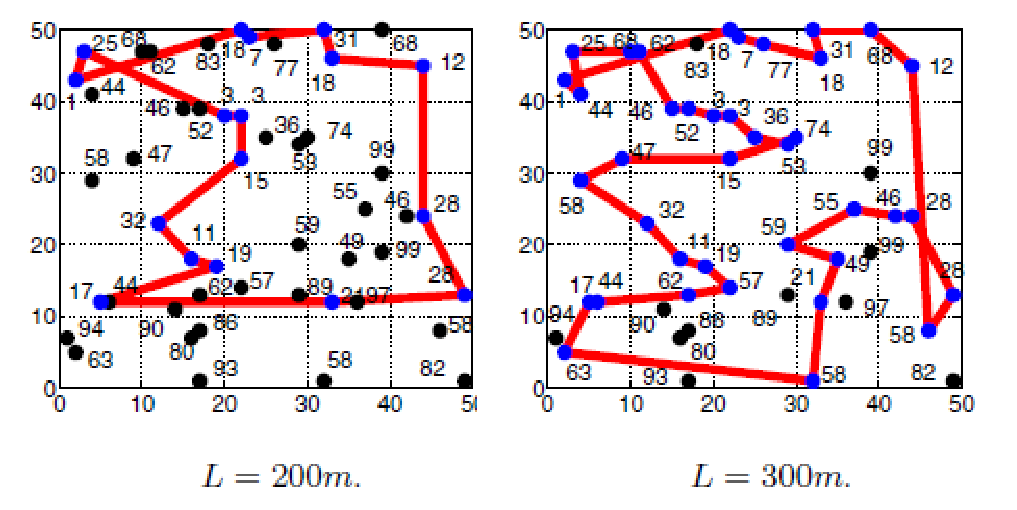
\includegraphics[width=0.8\textwidth]{images/yuanyuan_recharg_paths.eps}
	\caption{Δεξιά καλύφθηκε μεγαλύτερη διαδρομή αλλά ο κάθε κόμβος ξεχωριστά φορτίστηκε λιγότερο}
	\label{fig:yuanyuan_recharg_paths}
\end{figure}
Όπως φαίνεται και στην εικόνα \ref{fig:yuanyuan_recharg_paths} όσα περισσότερα σημεία εισαχθούν στο μονοπάτι που θα ακολουθήσει η κινητή οντότητα, τότε θα
υπάρχει μεγαλύτερη χρονοκαθυστέρηση (latency) στην συλλογή δεδομένων των στατικών κόμβων. Επομένως θα πρέπει να υπάρχει εξισορρόπηση ανάμεσα στην χρονοκαθυστέρηση και
στους κόμβους που θα φορτιστούν. Για να το πετύχουν αυτό, οι συγγραφείς απαιτούν από κάθε στατικό κόμβο να στείλει λίγο πριν το τέλος του γύρου την τρέχουσα ενέργειά
του. Αφού μαζευτούν όλες οι τρέχουσες ενέργειες των κόμβων στην κινητή οντότητα, αυτή τις διατάσει σε αύξουσα σειρά και ανάλογα με το όριο της διαδρομής επιλέγει τους
$L$ πρώτους κόμβους. Στην συνέχεια εφαρμόζεται ένας προσεγγιστικός αλγόριθμος TSP ο οποίος βρίσκει μία καλή διαδρομή για τα σημεία που επιλέχθηκαν. Για τον τρόπο
(μονοπάτι) με τον οποίο οι στατικοί κόμβοι επιλέγουν να στείλουν τα δεδομένα τους, οι συγγραφείς καταστρώνουν ένα γραμμικό πρόγραμμα το οποίο στη συνέχει το λύνουν
με έναν κατανεμημένο προσεγγιστικό αλγόριθμο. Οι προσομοιώσεις δείξαν οτι υπάρχει δραματική αυξηση του χρόνου ζωής του δικτύου σε σχέση με ασύρματα δίκτυα αισθητήρων
τα οποία χρησιμοποιούν εναλλακτικές μορφές ενέργειας.


Από τις παραπάνω δημοσιεύσεις μόνο οι \cite{prolonging_j-roc}, \cite{j-roc}, \cite{yuanyuan_joint} \cite{immortal_wsns} προσπαθήσουν να
λύσουν το πρόβλημα ενώ μόνο η \cite{yuanyuan_joint} χρησιμοποιεί κατανεμημένο αλγόριθμο αλλά  καμία από τις λύσεις που προτείνονται δεν χρησιμοποιεί τοπική
πληροφορία. Αντίθετα όλοι οι αλγόριθμοι που προτείνονται χρησιμοποιούν πληροφορίες από όλους τους κόμβους του δικτύου. Αυτό αποτελεί πρόβλημα καθώς σπαταλάται πολύ
ενέργεια σε μεγάλα δίκτυα. Επίσης δεν μελετώνται άλλα, πιο γενικά, θέματα όπως η γενική απόδοση του φορτιστή σε σχέση με την διαθέσιμη ενέργεια του δικτύου, η
αναλογία διαθέσιμης ενέργειας του φορτιστή σε σχέση με την διαθέσιμη ενέργεια των στατικών κόμβων αλλά και στρατηγικές φόρτισης που θα μπορούσαν να ωφελήσουν την
χρονοζωή (lifetime) του δικτύου.

\section{Στρατηγικές Επίλυσης}
Προκειμένου να λυθεί το CDDP πρόβλημα αποδοτικά, θα εφαρμοστούν ορισμένες στρατηγικές επίλυσης οι οποίες έχουν να κάνουν με συμβιβασμούς στην διαθέσιμη ενέργεια του
φορτιστή και των κόμβων.

\subsection{Ολική και Μερική Φόρτιση}
Κάθε φορά που ο φορτιστής $MC$ επισκέπτεται έναν κόμβο, μία αφελής στρατηγική θα ήταν να τον φορτίζει πλήρως τον κόμβο αυτό. Με αυτόν τον τρόπο ο $MC$ θα μπορούσε να
μεγιστοποιήσει τον χρόνο που χρειάζεται μέχρι να επιστρέψει στον ίδιο κόμβο και να τον ξαναφορτίσει για να μην εξαντληθεί όλη του η ενέργειά. Ωστόσο, καθώς το δίκτυο
λειτουργεί, υπάρχει κατανάλωση ενέργειας από τους κόμβους μέσα από την αποστολή μηνυμάτων αλλά και από τον ίδιο φορτιστή μέσα από την διαδικασία φόρτισης. Επομένως ο
φορτιστής θα έχει όλο και λιγότερη ενέργεια διαθέσιμη να δώσει στους κόμβους που την έχουν ανάγκη οι οποίοι με τον χρόνο θα αυξάνονται.

Μία διαφορετική στρατηγική για τον φορτιστή είναι να απλώσει συνετά την πολύτιμη ενέργειά του σε όσους περισσότερους κόμβους είναι δυνατόν προκειμένου να επεκτείνει
τον χρόνο ζωής του δικτύου. Ακολουθώντας αυτή την λογική, το ποσό της ενέργειας ο φορτιστής $MC$ παραδίδει σε έναν κόμβο είναι ανάλογο της διαθέσιμης ενέργειας του
ίδιου του φορτιστή. Δηλαδή, ο $MC$ φορτίζει έναν κόμβο μέχρι η ενέργειά του να γίνει:
\begin{align*}
e_{i} \approx \frac{E^{curr}_{MC}}{E^{init}_{MC}}\cdot E^{max}_{sensor}
\end{align*}

Προκειμένου να καθοριστεί η βέλτιστη στρατηγική φόρτισης στο κεφάλαιο \ref{ch:results} εκτελούνται μια σειρά πειραμάτων τα οποία συγκρίνουν την στρατηγική της ολικής
φόρτισης και την στρατηγική της προσαρμοστικής, μερικής φόρτισης. Τα πειραματικά αποτελέσματα δείχνουν οτι η μερική φόρτιση είναι πιο αποδοτική από την ολική φόρτιση.

\subsection{Ποσοστό Ενέργειας στον Φορτιστή}
Για να υπάρχει σωστή εκτίμηση της απόδοσης του φορτιστή, θεωρείται οτι η αρχική διαθέσιμη ενέργεια του δικτύου είναι $E_{total}$ και είναι πεπερασμένη και σταθερή
για όλες τις περιπτώσεις. Δηλαδή, λόγω του \ref{total} η $E_{total}$, ανάλογα σε κάθε περίπτωση, διαμοιράζεται ανάμεσα στον φορτιστή και τους κόμβους του δικτύου. Με
αυτόν τον τρόπο θα είναι δυνατόν να διερευνηθεί καλύτερα αν οι μετρικές του δικτύου έχουν καλύτερη απόδοση με ή χωρίς τον φορτιστή και την διαδικασία φόρτισης. Αυτός
ο συγκεκριμένος συμβιβασμός έχει σχέση με το ποσό της ενέργεια (σε σχέση με την ολική ενέργεια $E_{total}$) το οποίο θα διοχετευθεί αρχικά στον φορτιστή $MC$.
Περισσότερη ενέργεια στον φορτιστή θα οδηγήσει σε καλύτερη διαχείρηση της ενέργειας στο δίκτυο, αφού ο φορτιστής μπορεί να δώσει την ενέργεια εκεί που πραγματικά
χρειάζεται (π.χ. σε ένα κρίσιμο μονοπάτι). Ωστόσο, λόγω της \ref{total} περισσότερη ενέργεια στον $MC$ θα σήμαινε οτι οι κόμβοι ξεκινάνε στο δίκτυο με μικρότερη
αρχική ενέργεια, δηλαδή χωρίς να είναι πλήρως φορτισμένοι. Έτσι, θα είναι πολύ πιθανόν οτι θα τους τελειώσει η ενέργεια πριν ο φορτιστής $MC$ τους φορτίσει,
οδηγόντας έτσι σε πιθανές αποσυνδέσεις του δικτύου και χαμηλή κάλυψη της περιοχής από τους κόμβους.

Προκειμένου να καθοριστεί η βέλτιση κατανομή ενέργειας ανάμεσα στον φορτιστή και τους κόμβους στο κεφάλαιο \ref{ch:results} εκτελούνται μια σειρά από πειράματα με
διάφορες αναλογίες ανάμεσα στην αρχική διαθέσιμη ενέργεια των κόμβων, $E_{sensors}$ και την αρχική διαθέσιμη ενέργεια του φορτιστή, $E^{init}_{MC}$. Όπως θα φανεί στο
κεφάλαιο \ref{ch:results} η βέλτιστη αναλογία που βρέθηκε πειραματικά είναι 20\% της αρχικής ενέργειας $E_{total}$ να δοθεί στον φορτιστή και το υπόλοιπο 80\% της
ενέργειας να δοθεί στους κόμβους.

\subsection{Διαδρομές του Φορτιστή}
Η αποδοτική διαχείρηση της ενέργειας σε ένα ασύρματο δίκτυο αισθητήρων εξαρτάται σημαντικά και από τις διαδρομές που ακολουθεί ο φορτιστής. Παρακάτω παρουσιάζεται
αρχικά μια διαδρομή η οποία έχει πλήρη γνώση (global knowledge) της κατάστασης του δικτύου, 3 διαδρομες οι οποίες χρησιμοποιούν μόνο τοπική πληροφορία ενώ η
τελευταία που παρουσιάζεται όχι μόνο χρησιμοποιεί τοπική πληροφορία αλλά ταυτόχρονα έχει και προσαρμοστικό χαρακτήρα ανάλογα με την κατάσταση του δικτύου.

\subsubsection{Φορτιστής με Καθολική Γνώση}
Ο φορτιστής καθολικής γνώσης (global-knowledge charger) ο οποίο μελετάται, αποτελεί ουσιαστικά έναν αλγόριθμο άμεσης απόκρισης (online algorithm) ο οποίο σε κάθε γύρο
ελαχιστοποιεί το γινόμενο της ενέργειας του κάθε κόμβου με την απόστασή του από την τρέχουσα θέση του φορτιστή. Πιο συγκεκριμένα, σε κάθε γύρο ο φορτιστής καθολικής
γνώσεις ελαχιστοποιεί το ακόλουθο γινόμενο:
\begin{align*}
P = min\left\{ \left(1 + \frac{E_{curr}}{E_{init}}\right) \cdot \left(1  + \frac{dist_{curr}}{2R}\right) \right\}
\end{align*}
όπου $E_{curr}$, $E_{init}$  και $dist_{curr}$ είναι αντίστοιχα η τρέχουσα ενέργεια, η αρχική ενέργεια και η απόσταση του κάθε κόμβου. Η ελάχιστη τιμή λαμβάνεται
αφού γίνει η σύγκριση σε όλους τους κόμβους. Αφού η στρατηγική αυτή απαιτεί καθολική γνώση της κατάστασης του δικτύου, είναι αναμενόμενο να υπερτερεί κάθε άλλου
αλγορίθμου που χρησιμοποιεί τοπική γνώση. Ωστόσο, τέτοιοι αλγόριθμοι δεν είναι καταλληλοι για πραγματικά δίκτυα και δεν έχει καλή κλιμακωσιμότητα καθώς εισάγει
πολύ μεγάλο επικοινωνιακό κόστος αφού κάθε κόμβος θα πρέπει να διαδόσει την τρέχουσα ενέργειά του σε κάθε γύρο.


\subsubsection{Σπειροειδης Φορτιστής}
Ο σπειροειδης φορτιστής ξεκινάει από την Πηγή και διανύει διαδρομή η οποία σχηματίζει ομόκεντρους κύκλους με κέντρο την Πηγή αλλά με αυξανόμενη ακτίνα. Επομένως
σχηματίζει μία σπείρα μέχρις ότου φτάσει τα ακριανά όρια της περιοχής του δικτύου. Στην συνέχεια  ο $MC$ ακολουθεί την ίδια διαδρομή αλλά με αντίθετη κατεύθυνση. Τα
πλεονεκτήματα αυτής της κίνησης είναι οτι η σπείρα είναι ο μόνος ντεντερμινιστικός αλγόριθμος ο οποίος μπορεί να καλύψει όλο το δίκτυο δίκαια, δηλαδή σχεδόν όλοι οι
κόμβοι φορτίζονται από τον $MC$ μέχρι να τελειώσει η διαθέσιμη ενέργειά του. Όμως, αυτή η κίνηση δεν είναι προσαρμοστική, δηλαδή δεν  λαμβάνει υπόψην διαφορές στον
ρυθμό κατανάλωσης των κόμβων οι οποίες προκλήθηκαν από το εκάστοτε πρωτόκολλο δρομολόγησης που τρέχει.

\subsubsection{Διαμετρικός Φορτιστής}
Ο διαμετρικός φορτιστής αρχικά ξεκινάει από την Πηγή και επιλέγει τυχαία μια κατεύθυνση την οποία ακολουθεί μέχρι να φτάσει στα όρια της περιοχής του δικτύου, δηλαδή
κινείται πάνω στην αντίστοιχη διάμετρο του δικτύου. Στην συνέχεια αφού έχει φτάσει στην περίμετρο του δικτύου, κινείται πάνω στην περίμετρο της περιοχής του δικτύου
για $d$ μοίρες, δηλαδή διανύει απόσταση ίση με $\frac{d}{2\pi}2\pi R = d\cdot R$ επάνω στην περίμετρο. Στην συνέχεια ξεκινάει να κινείται επάνω στην αντίστοιχη
διάμετρο του δικτύου εως ότου φτάσει στην αντιδιαμετρική άκρη του δικτύου. Αυτή η διαδικασία συνεχίζεται μέχρι να τελειώσει η εναπομείνουσα ενέργεια του φορτιστή.
Προκειμένου οι διαδρομές που ακολουθεί ο φορτιστής να μην επικαλύπτονται, σε κάθε βήμα το $d$ επιλέγεται τυχαία ομοιόμορφα στο διάστημα $(0,90]$ μοιρών. Ακολουθώντας
αυτή την διαδρομή ο $MC$ καταφέρνει να φορτίσει όλους τους κόμβους που βρίσκονται μακριά αλλά και κοντά στην Πηγή. Ωστόσο, παρ'όλο που η διαδρομή είναι απλή, δεν
είναι προσαρμοστική. Ένα στιγμιότυπο της διαδρομής φαίνεται στην εικόνα \ref{fig:diameter_charger}.
\vspace{0.9cm}
\begin{figure}[h]
	\centering
	\includegraphics[width=0.3\textwidth]{images/diameter.eps}
	\caption{Ένα στιγμιότυπο του Διαμετρικού Φορτιστή.}
	\label{fig:diameter_charger}
\end{figure}


\subsubsection{Φορτστής σε Τυχαίο Περίπατο}
Ο φορτιστής σε τυχαίο περίπατο ακολουθεί τον τυφλό τυχαίο περίπατο (blind random walk). Σε κάθε νέο γύρο, η επόμενη κίνηση του φορτιστή είναι τυχαία, στοχαστικά
ανεξάρτητη από κάθε προηγούμενη επιλογή. Δεδομένου της τρέχουσας θέσης του φορτιστή, έστω ο κόμβος $i$ τότε η πιθανότητα μετάβασης σε οποιονδήποτε γείτονα $j$ του
κόμβου $i$ είναι $p_{i,j} =\frac{1}{deg(i)}$. Η τροχία αυτή είναι πολύ αποδοτική ως προς την έννοια οτι πιθανοτικά εγγυάται οτι τελικά όλο η περιοχή του δικτύου θα
καλυφθεί και όλοι οι κόμβοι θα επισκεφθούν Ωστόσο μπορεί να γίνει αποδοτική σε δίκτυα με περιοχές συμφόρησης ή με ειδικούς κόμβους (όπως κόμβους αρχηγούς σε
ιεραρχικά πρωτόκολλα) και γενικά σε δίκτυα που υπάρχουν κόμβοι που εξυπηρετούν μεγαλύτερη κίνηση από άλλους κόμβους όπως συμβαίνει σε πολυ-βηματικά (multi-hop)
πρωτόκολλα.

\subsubsection{Προσαρμοστικός Φορτιστής}
Δεδομένου της συμμετρίας του δικτύου, της ομοιόμορφης κατανομής, και της ομοιόμορφης γέννησης μηνυμάτων του δικτύου ο πρασαρμοστικός φορτιστής ακολουθεί μια κυκλική
τροχιά με κέντρο την Πηγή η οποία βρίσκεται στο κέντρο του δικτύου. Η ακτίνα της κυκλικής τροχιάς ποικίλει και προσαρμόζεται στην κατανάλωση ενέργειας της κάθε
υποπεριοχής του δικτύου. Έστω $S$ το σύνολο αυτών των κόμβων όπου $|S| = 2\pi R_{MC}\cdot \rho$. Έστω, επίσης, $e_{i}$ οτι δηλώνει την τρέχουσα ενέργεια του κόμβου
$i$. Ξεκινώντας από την Πηγή, ο κινητός φορτιστής διανύει μια διαδρομή η οποία σχηματίζει ομόκεντρους κύκλους με κέντρο την ίδια την Πηγή αλλά με ακτίνα η οποία
αυξάνεται ή μειώνεται ανάλογα. Σε μια δεδομένη απόσταση από την Πηγή ο προσαρμοστικός φορτιστής καταγράφει την μέση τιμή της ενέργειας των κόμβων οι οποίοι
βρίσκονται επάνω στην αντίστοιχη κυκλική τροχιά. Έστω η μέση ενέργεια όλων των κόμβων οτι είναι $\overline{E}_{current}$. Αντίστοιχα ο προσαρμοστικός φορτιστής
κρατάει στην μνήμη του την μέση τιμή της ενέργειας των κόμβων που βρίσκονταν στην προηγούμενη κυκλική τροχιά του, έστω $\overline{E}_{previous}$. Χρησιμοποιώντας
αυτές τις 2 τιμές ο προσαρμοστικός φορτιστής βελτιστοποιεί την κυκλική τροχιά του με κριτήριο την φόρτιση των κόμβων οι οποίοι καταναλώνουν την ενέργειά τους πιο
γρήγορα.

Ο αλγόριθμος που εκτελεί ο προσαρμοστικός φορτιστής φαίνεται παρακάτω:
\vspace{0.1cm}
\begin{algorithm}
\begin{algorithmic}
\caption{Προσαρμοστικός Φορτιστής}
\While{$E_{MC}^{curr} > 0$}
\State $E_{tmp}=0$
\For{every $i\in S$}
\State $E_{tmp}+=e_{i}^{c}$
\State Charge until $e_{i} \approx \frac{E_{MC}^{curr}}{E_{MC}^{init}}\cdot E_{sensor}^{max}$
\EndFor
\State $\overline{E}_{current}=\frac{E_{tmp}}{|S|} = \frac{\sum e_{i}}{|S|}$
\If {$\overline{E}_{current} \approx \overline{E}_{init}$}
    \If {$\overline{E}_{previous} \geq \overline{E}_{current}$ }
		\State	Keep direction
	\Else
		\State Change direction
	\EndIf
\EndIf
\EndWhile
\end{algorithmic}
\end{algorithm}

Ο προσαρμοστικός φορτιστής $MC$ ξεκινάει να διασχίζει το δίκτυο από το κέντρο του θέτοντας $R_{MC}=1$, δηλαδή θα επισκεφθεί όλους τους κόμβους που βρίσκονται 1-βήμα
(1-hop) μακριά από την Πηγή. Μόλις όλοι αυτοί οι κόμβοι φορτιστούν, δηλαδή οι κόμβοι που συναντά ο $MC$ έχουν ενέργεια $e_{i} = E^{max}_{sensor}$ ο $MC$ αυξάνει την
ακτίνα του $R_{MC}$ επισκέπτοντας τους κόμβους που είναι 2-βήματα (2-hop) μακριά από την Πηγή. Συγκρίνοντας τις τιμές $\overline{E}_{current}$ και
$\overline{E}_{previous}$ ο $MC$ μπορεί να καταλάβει προς ποια περιοχή θα κινηθεί, δηλαδή προς την περιοχή η οποία έχει μεγαλύτερη κατανάλωση ενέργεια. Συγκεκριμένα,
αν $\overline{E}_{current} < \overline{E}_{previous}$ τότε ο $MC$ υποθέτει οτι κινείται προς την σωστή περιοχή, δηλαδή αυτή στην οποία υπάρχει μεγάλο φορτίο.
Αντίθετα αν $\overline{E}_{current} > \overline{E}_{previous}$ τότε ο $MC$ αμέσως καταλαβαίνει οτι κινείται προς την λάθος περιοχή και έτσι αλλάζει κατεύθυνση.

